\documentclass[a4paper,10pt,DIV=14]{article}
\usepackage{graphicx}
\usepackage[utf8]{inputenc} % korrekte Darstellung von Umlauten u. Sonderzeichen
\usepackage[ngerman]{babel} % Sprachpaket, ngerman = neue deutsche Rechtschreibung
\usepackage{amsmath} % Setzen mathematischer Formeln
\usepackage{amsfonts} %mathbb
\usepackage{titlesec}
\usepackage{float}
\usepackage{caption}
\usepackage{fancyvrb}
\usepackage{siunitx}
\usepackage{booktabs}
\usepackage{enumitem}
\usepackage{tikz}
\usetikzlibrary{positioning}

\usepackage{subcaption}


\usepackage{tikz}
\usetikzlibrary{3d}
\usetikzlibrary{shadings}
\definecolor{mypurple}{RGB}{255,0,255}

\makeatletter
\tikzoption{canvas is xy plane at z}[]%
{   \def\tikz@plane@origin{\pgfpointxyz{0}{0}{#1}}%
	\def\tikz@plane@x{\pgfpointxyz{1}{0}{#1}}%
	\def\tikz@plane@y{\pgfpointxyz{0}{1}{#1}}%
	\tikz@canvas@is@plane
}
\makeatother 

\usepackage{tabularx}
\newcolumntype{L}[1]{>{\raggedright\arraybackslash}p{#1}} % linksbündig mit Breitenangabe
\newcolumntype{C}[1]{>{\centering\arraybackslash}p{#1}} % zentriert mit Breitenangabe
\newcolumntype{R}[1]{>{\raggedleft\arraybackslash}p{#1}} % rechtsbündig mit Breitenangabe

\newcommand{\gqq}[1]{\glqq{}#1\grqq{}}
\newcommand{\gq}[1]{\glq{}#1\grq{}}
\newcommand{\dg}[1]{#1^\circ}

\renewcommand{\thesection}{Aufgabe \arabic{section}:}
\renewcommand{\thesubsection}{\alph{subsection})}
\renewcommand{\thesubsubsection}{\roman{subsubsection}}

\titleformat{\subsection}
{\normalsize}{\thesubsection}{1em}{}


\captionsetup[figure]{labelformat=empty}

\begin{document}

\title{Graphische Datenverarbeitung WS17/18 \\ Theorieübung 4}
\author{
  Salmah Ahmad (2880011)
  \and
  Markus Höhn (1683303)
  \and
  Tobias Mertz (2274355)
  \and
  Steven Lamarr Reynolds (1620638)
  \and
  Sascha Zenglein (2487032)
}

\maketitle

\section{Beleuchtung (4 Punkte)}

\subsection{(1 Punkt)}

\subsubsection{}

Umrechnung von RGB in HSV: \\
\newline
$
R' = R/255\\
G' = G/255\\
B' = B/255\\
max = max((R', G', B'))\\
min = min((R', G', B'))\\
\Delta = max - min
$\\~\\
$
H = \begin{cases}
0^\circ &\Delta = 0\\
60^\circ \times (\frac{G'-B'}{\Delta}) &, max = R'\\
60^\circ \times (\frac{B'-R'}{\Delta}+2) &, max = G'\\
60^\circ \times (\frac{R'-G'}{\Delta}+4) &, max = B'\\
\end{cases}
$\\~\\~\\
$
S = \begin{cases}
0 & max = 0\\
\frac{\Delta}{max}, &max \neq 0\\
\end{cases}
$\\~\\~\\
$
V = max
$\\

$
\text{Grün}_{HSV} = (120^\circ, 1, 1)
$\\
$
\text{Magenta}_{HSV} = (300^\circ, 1, 1)
$

\subsubsection{}

$
f_{RGB}(x) = ((1-x)\cdot255, \ x\cdot255, \ (1-x)\cdot255)
$\\
$
f_{HSV} = ((1-x)\cdot300^\circ + x\cdot 120^\circ, \ 1, \ 1)
$

\subsubsection{}

RGB Cube:\\

\pgfmathtruncatemacro{\Divisions}{30}
\pgfmathsetmacro{\Cube}{3}

\begin{tikzpicture}
[   x={(0.5cm,0.5cm)},
y={(0.95cm,-0.25cm)},
z={(0cm,0.9cm)}
]
\begin{scope}[canvas is yz plane at x=-\Cube/2] %front
\shade[lower right=mypurple, lower left=blue, upper right=white, upper left=cyan] (-1,-1) rectangle (1,1);
\clip (-\Cube/2,-\Cube/2) rectangle (\Cube/2,\Cube/2);
\colorlet{BL}[RGB]{blue}
\colorlet{BR}[RGB]{mypurple}
\colorlet{TL}[RGB]{cyan}
\colorlet{TR}[RGB]{white}
\foreach \x in {1,...,\Divisions}
{   \pgfmathtruncatemacro{\px}{(\x-1)/(\Divisions-1)*100}
	\colorlet{B}[RGB]{BR!\px!BL}
	\colorlet{T}[RGB]{TR!\px!TL}
	\foreach \y in {1,...,\Divisions}
	{   \pgfmathtruncatemacro{\py}{(\y-1)/(\Divisions-1)*100}
		\fill[T!\py!B] ({-\Cube/2+\Cube*(\x-1)/\Divisions},{-\Cube/2+\Cube*(\y-1)/\Divisions}) rectangle ({-\Cube/2+\Cube*(\x+0.1)/\Divisions},{-\Cube/2+\Cube*(\y+0.1)/\Divisions});
	}
}
\draw (-\Cube/2,-\Cube/2) rectangle (\Cube/2,\Cube/2);
\end{scope}

\begin{scope}[canvas is xz plane at y=\Cube/2] %right
\clip (-\Cube/2,-\Cube/2) rectangle (\Cube/2,\Cube/2);
\colorlet{BL}[RGB]{mypurple}
\colorlet{BR}[RGB]{red}
\colorlet{TL}[RGB]{white}
\colorlet{TR}[RGB]{yellow}
\foreach \x in {1,...,\Divisions}
{   \pgfmathtruncatemacro{\px}{(\x-1)/(\Divisions-1)*100}
	\colorlet{B}[RGB]{BR!\px!BL}
	\colorlet{T}[RGB]{TR!\px!TL}
	\foreach \y in {1,...,\Divisions}
	{   \pgfmathtruncatemacro{\py}{(\y-1)/(\Divisions-1)*100}
		\fill[T!\py!B] ({-\Cube/2+\Cube*(\x-1)/\Divisions},{-\Cube/2+\Cube*(\y-1)/\Divisions}) rectangle ({-\Cube/2+\Cube*(\x+0.1)/\Divisions},{-\Cube/2+\Cube*(\y+0.1)/\Divisions});
	}
}
\draw (-\Cube/2,-\Cube/2) rectangle (\Cube/2,\Cube/2);
\end{scope}

\begin{scope}[canvas is xy plane at z=\Cube/2] %top
\clip (-\Cube/2,-\Cube/2) rectangle (\Cube/2,\Cube/2);
\colorlet{BL}[RGB]{cyan}
\colorlet{BR}[RGB]{green}
\colorlet{TL}[RGB]{white}
\colorlet{TR}[RGB]{yellow}
\foreach \x in {1,...,\Divisions}
{   \pgfmathtruncatemacro{\px}{(\x-1)/(\Divisions-1)*100}
	\colorlet{B}[RGB]{BR!\px!BL}
	\colorlet{T}[RGB]{TR!\px!TL}
	\foreach \y in {1,...,\Divisions}
	{   \pgfmathtruncatemacro{\py}{(\y-1)/(\Divisions-1)*100}
		\fill[T!\py!B] ({-\Cube/2+\Cube*(\x-1)/\Divisions},{-\Cube/2+\Cube*(\y-1)/\Divisions}) rectangle ({-\Cube/2+\Cube*(\x+0.1)/\Divisions},{-\Cube/2+\Cube*(\y+0.1)/\Divisions});
	}
}
\draw (-\Cube/2,-\Cube/2) rectangle (\Cube/2,\Cube/2);
\end{scope}
\draw [-stealth](-\Cube/2,\Cube/2, -\Cube/2) -> (\Cube/2,-\Cube/2, \Cube/2);
\end{tikzpicture}\\


HSV Cone: \\
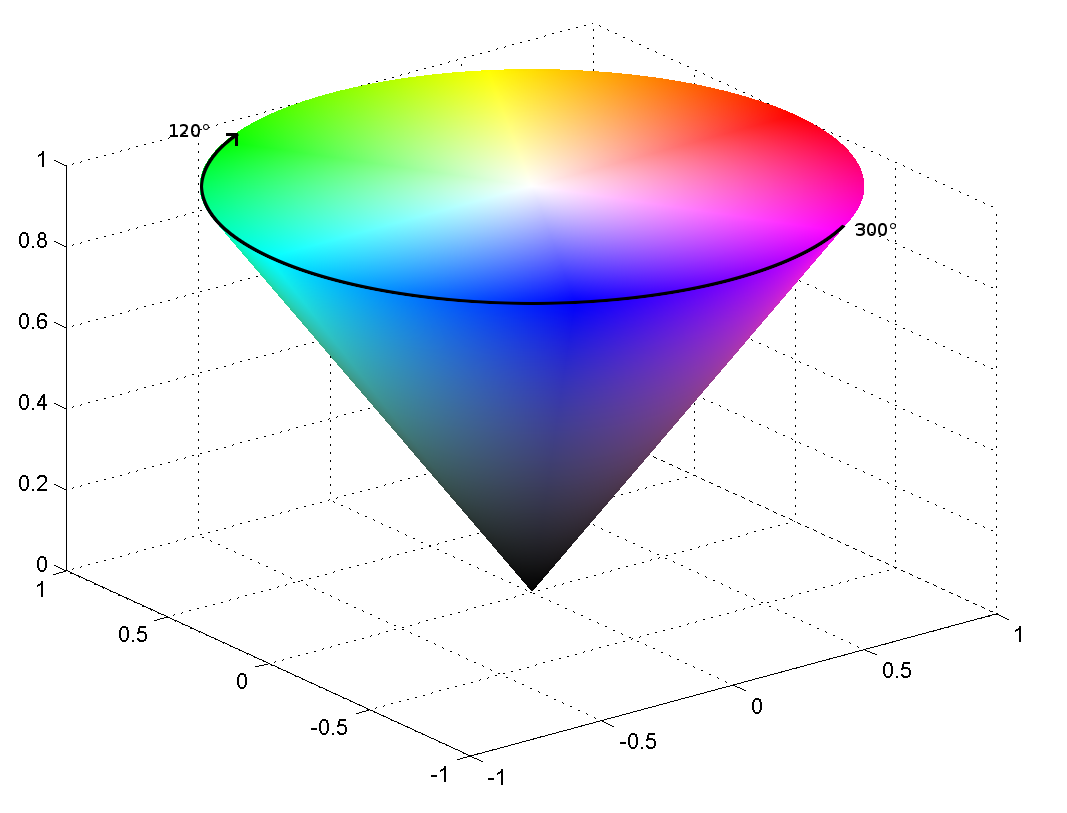
\includegraphics[scale=0.5]{hsv}

\subsubsection{}

\definecolor{rgb1}{RGB}{204, 51, 204}
\definecolor{rgb2}{RGB}{153, 102, 153}
\definecolor{rgb3}{RGB}{128, 128, 128}
\definecolor{rgb4}{RGB}{102, 153, 102}
\definecolor{rgb5}{RGB}{51, 204, 51}

\definecolor{hsv1}{RGB}{102, 0, 255}
\definecolor{hsv2}{RGB}{0, 51, 255}
\definecolor{hsv3}{RGB}{0, 128, 255}
\definecolor{hsv4}{RGB}{0, 204, 255}
\definecolor{hsv5}{RGB}{0, 255, 153}

$
x_1 = 0.2\\
x_2 = 0.4\\
x_3 = 0.5\\
x_4 = 0.6\\
x_5 = 0.8\\~\\
f_{RGB}(x_1) = (204, 51, 204)\tikz \fill [rgb1] (0.1,0.1) rectangle (0.4,0.4);\\
f_{RGB}(x_2) = (153, 102, 153)\tikz \fill [rgb2] (0.1,0.1) rectangle (0.4,0.4);\\
f_{RGB}(x_3) = (127.5, 127.5, 127.5)\tikz \fill [rgb3] (0.1,0.1) rectangle (0.4,0.4);\\
f_{RGB}(x_4) = (102, 153, 102)\tikz \fill [rgb4] (0.1,0.1) rectangle (0.4,0.4);\\
f_{RGB}(x_5) = (51, 204, 51)\tikz \fill [rgb5] (0.1,0.1) rectangle (0.4,0.4);\\~\\
f_{HSV}(x_1) = (264^\circ, 1, 1)\tikz \fill [hsv1] (0.1,0.1) rectangle (0.4,0.4);\\
f_{HSV}(x_2) = (228^\circ, 1, 1)\tikz \fill [hsv2] (0.1,0.1) rectangle (0.4,0.4);\\
f_{HSV}(x_3) = (210^\circ, 1, 1)\tikz \fill [hsv3] (0.1,0.1) rectangle (0.4,0.4);\\
f_{HSV}(x_4) = (192^\circ, 1, 1)\tikz \fill [hsv4] (0.1,0.1) rectangle (0.4,0.4);\\
f_{HSV}(x_5) = (156^\circ, 1, 1)\tikz \fill [hsv5] (0.1,0.1) rectangle (0.4,0.4);\\~\\
$

\subsection{(1 Punkt)}

\subsection{(1 Punkt)}%c
\newcommand{\VecThree}[3]{\begin{pmatrix} #1 \\ #2 \\ #3 \end{pmatrix}}
Gegeben:
\begin{gather*}
N = \VecThree{0}{1}{0}, V = \VecThree{\sqrt{0.5}}{\sqrt{0.5}}{0}, H = \VecThree{\frac{\sqrt{6}}{6}}{\frac{\sqrt{6}}{3}}{-\frac{\sqrt{6}}{6}}, \lVert L+V \rVert = \sqrt{3}, k = 1, I_{BP} = \frac{\sqrt{6}}{3}
\end{gather*}
\\
\begin{gather*}
I_p = f_p(\gamma) = (R(L)^T \cdot V)^k \cdot E = cos^k(\gamma) \cdot E \\
I_{BP} = f_{BP}(\phi) = (H^T \cdot N)^k \cdot E = cos^k(\phi) \cdot E = \frac{\sqrt{6}}{3} \\
\end{gather*}
\begin{gather*}
E = \frac{\frac{\sqrt{6}}{3}}{(H^T \cdot N)^k} = \frac{\sqrt{6} \cdot (H^T \cdot N)^k}{3} \\
= \frac{\sqrt{6} \cdot \left(\VecThree{\frac{\sqrt{6}}{6}}{\frac{\sqrt{6}}{3}}{-\frac{\sqrt{6}}{6}}^T \cdot \VecThree{0}{1}{0}\right)^1}{3} = \frac{\sqrt{6} \cdot \frac{\sqrt{6}}{3}}{3} =  \frac{2}{3}
\end{gather*}
\\
\begin{gather*}
\gamma = \arccos(R(L)^T \cdot V) \\
= \arccos\left(\VecThree{0}{\sqrt{0.5}}{\frac{\sqrt{2}}{2}} \cdot \VecThree{\sqrt{0.5}}{\sqrt{0.5}}{0} \right) \\
= \arccos(0.5) \approx 1.047
\end{gather*}
\\
\begin{gather*}
I_p = cos(\gamma) \cdot E = 0.5 \cdot E = \frac{1}{3}
\end{gather*}
\\
\begin{gather*}
\phi = \arccos(H^T \cdot N) = \arccos\left(\frac{\sqrt{6}}{3}\right) \approx 0.615
\end{gather*}
\\
\begin{gather*}
\lVert L+V \rVert = \VecThree{l_1}{l_2+1}{l_3} = \sqrt{l_1^2 + (l_2+1)^2 + l_3^2} = \sqrt{3} \\
l_1^2 + (l_2+1)^2 + l_3^2 = 3
\end{gather*}
\\
\begin{gather*}
R(L) = - L + 2 \left(L \cdot N \right) N \\
= - \VecThree{0}{\sqrt{0.5}}{-\frac{\sqrt{2}}{2}} + 2 \left(\VecThree{0}{\sqrt{0.5}}{-\frac{\sqrt{2}}{2}} \cdot \VecThree{0}{1}{0} \right) \VecThree{0}{1}{0} \\
= - \VecThree{0}{\sqrt{0.5}}{-\frac{\sqrt{2}}{2}} + 2 \left( \sqrt{0.5} \right) \VecThree{0}{1}{0} \\ 
= \VecThree{0}{\sqrt{0.5}}{\frac{\sqrt{2}}{2}}
\end{gather*}
\\
\begin{align*}
H &= \frac{L+V}{\lVert L+V \rVert} = \frac{L+V}{\sqrt{3}} \\
\VecThree{\frac{\sqrt{6}}{6}}{\frac{\sqrt{6}}{3}}{-\frac{\sqrt{6}}{6}} &= \frac{L+V}{\sqrt{3}} \\
L &= \VecThree{\frac{\sqrt{6}}{6}}{\frac{\sqrt{6}}{3}}{-\frac{\sqrt{6}}{6}} \cdot \sqrt{3} - \VecThree{\sqrt{0.5}}{\sqrt{0.5}}{0} = \VecThree{\frac{\sqrt{2}}{2}}{\sqrt{2}}{-\frac{\sqrt{2}}{2}} - \VecThree{\sqrt{0.5}}{\sqrt{0.5}}{0} = \VecThree{0}{\sqrt{0.5}}{-\frac{\sqrt{2}}{2}}
\end{align*}
\\
Lösung:
\begin{gather*}
E = \frac{2}{3} \\
I_P = \frac{1}{3}\\
\gamma = \arccos(0.5) \approx 1.047\\
\phi = \arccos\left(\frac{\sqrt{6}}{3}\right) \approx 0.615 \\
L =  \VecThree{0}{\sqrt{0.5}}{-\frac{\sqrt{2}}{2}} \\
R(L) = \VecThree{0}{\sqrt{0.5}}{\frac{\sqrt{2}}{2}}\\
\end{gather*}

\subsection{(0.5 Punkte)} %d
%TODO, auskommentiert damit niemand denkt es wäre fertig
%\begin{gather*}
%I_{BP} \neq 0 \neq I_P \\
%(R(L)^T \cdot V)^k = cos^k(\gamma) \\
%(H^T \cdot N)^k = cos^k(\phi) \\
%\gamma = \phi \\
%\Rightarrow \left\vert R(L)^T \cdot V \right\vert = \left\vert H^T \cdot N \right\vert \\
%\Rightarrow \left\vert \left(- L + 2 \left(L \cdot N \right) N\right)^T \cdot V \right\vert = \left\vert \left(\frac{L+V}{\lVert L+V \rVert}\right)^T \cdot N \right\vert
%\end{gather*}
\subsection{(0.5 Punkte)}

\section{Texturierung (2 Punkte)}

\subsection{(1 Punkt)}

\subsection{(1 Punkt)} 

\section{Perspektivisch korrekte Texturierung (4 Punkte)}

\subsection{(1 Punkt)}

\subsection{(1 Punkt)} 

\subsection{(1 Punkt)}

\subsection{(1 Punkt)}


\end{document}
